\documentclass[a5paper]{article}
\usepackage[a5paper, top=8mm, bottom=8mm, left=8mm, right=8mm]{geometry}

\usepackage{polyglossia}
\setdefaultlanguage[babelshorthands=true]{russian}

\usepackage{fontspec}
\setmainfont{FreeSerif}
\newfontfamily{\russianfonttt}[Scale=0.7]{DejaVuSansMono}

\usepackage[font=scriptsize]{caption}

\usepackage{amsmath}
\usepackage{amssymb,amsfonts,textcomp}
\usepackage{color}
\usepackage{array}
\usepackage{hhline}
\usepackage{cite}

\usepackage[hang,multiple]{footmisc}
\renewcommand{\footnotelayout}{\raggedright}

\PassOptionsToPackage{hyphens}{url}\usepackage[xetex,linktocpage=true,plainpages=false,pdfpagelabels=false]{hyperref}
\hypersetup{colorlinks=true, linkcolor=blue, citecolor=blue, filecolor=blue, urlcolor=blue, pdftitle=1, pdfauthor=, pdfsubject=, pdfkeywords=}

\usepackage{tabu}

\usepackage{graphicx}
\usepackage{indentfirst}
\usepackage{multirow}
\usepackage{subfig}
\usepackage{footnote}
\usepackage{minted}
\usepackage{xcolor}

\newcommand{\attribution}[1] {
\vspace{-5mm}\begin{flushright}\begin{scriptsize}\textcolor{gray}{\textcopyright\, #1}\end{scriptsize}\end{flushright}
}

\sloppy
\pagestyle{plain}

\title{Работа с сетью, низкий уровень}
\author{Юрий Литвинов\\\small{y.litvinov@spbu.ru}}

\date{05.10.2021}

\begin{document}

\maketitle
\thispagestyle{empty}

\section{Архитектура сетей}

Рассказ про сетевое программирование, наверное, стоило бы начать сразу с того, как данные по сети передавать, но в университетском курсе, как мне кажется, должно быть более фундаментальное образование, так что начнём с самого начала. Подробнее про то, как устроены сети, вам ещё расскажут на специально посвящённых этому курсах, у нас будет всего пара занятий про это, но понимать, что происходит, необходимо, чтобы работа с сетью не казалась магией. Понимать, к несчастью, приходится много чего, потому что <<под капотом>> сеть устроена довольно хитро. Поэтому сейчас может показаться, что материала очень много и сразу, но делать нечего. Постараюсь особо в подробности не вдаваться. За гораздо более плавным и подробным введением отправлю к классической книге Э. Таненбаум, Д.Уэзеролл. <<Компьютерные сети>> (откуда, кстати, будут позаимствованы многие изображения дальше).

Зачем нужны компьютерные сети и зачем их нужно обязательно уметь программировать, я думаю, объяснять людям, родившимся в 21 веке, уже не надо. Так что начнём сразу с того, как всё устроено. Вот картинка из книжки Таненбаума с общей архитектурой сети Интернет:
\begin{center}
    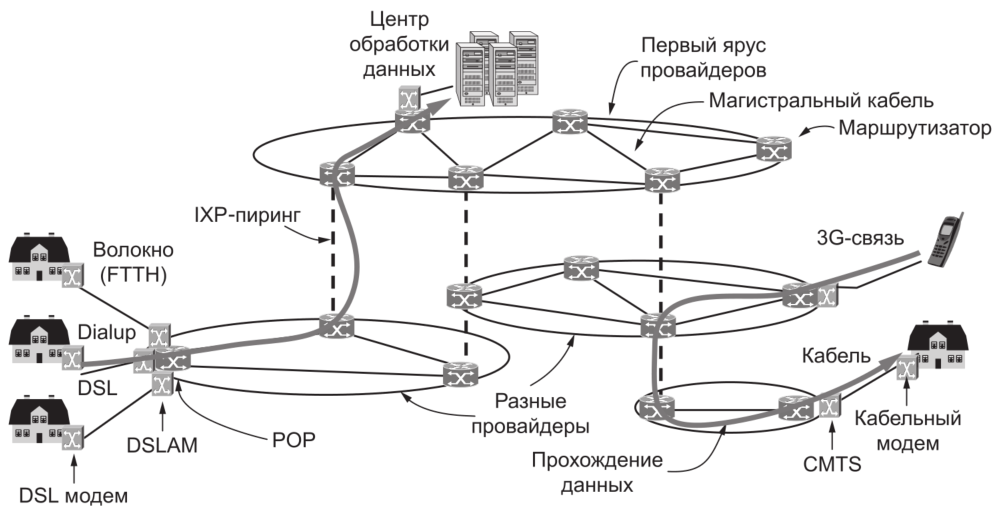
\includegraphics[width=0.9\textwidth]{internetArchitecture.png}
    \attribution{Э. Таненбаум}
\end{center}

Интернет --- это не единая сеть, а множество сетей разных провайдеров, соединённых в одну так, чтобы отовсюду из сети было доступно всё, что в этой сети находится. Как это работает: есть разные провайдеры, каждый из которых строит свою сеть, чаще всего, непосредственно до потребителей услуг (то есть обычных людей или организаций). При этом для подключения каждого абонента могут использоваться разные технологии. Сейчас это чаще всего Ethernet, бывают оптоволоконные линии; немного устарели, но иногда ещё встречаются DSL-модемы, и, разумеется, разные сорта радиоканалов --- обычный 3G через сеть мобильного оператора, LTE, WiMax. Суть в том, что так или иначе сеть позволяет абоненту общаться с оборудованием провайдера. В случае с Ethernet это обычно маршрутизатор, который стоит в электрощите на лестничной клетке, к нему подключаются все близлежащие абоненты, а из него выходит провод, идущий к следующему маршрутизатору провайдера. Провайдер, в свою очередь, каким бы большим и крутым ни был, не подключён непосредственно <<к интернету>> (просто потому, что такого понятия не существует), а пользуется услугами другого провайдера, и так далее до провайдеров самого высокого уровня, владеющих магистральными линиями, типа трансатлантических подводных кабелей или спутников. Провайдеры также могут соединяться с подсетями соседних провайдеров, чтобы совместно обрабатывать трафик, в этом случае бывает так, что никто никому не платит, а сети используются совместно. Соединение подсетей провайдеров происходит через Internet Exchange Point (IXP), которые представляют собой либо стойку с маршрутизаторами, либо целый датацентр, через который течёт трафик из одной подсети в другую. Есть ряд известных крупных IXP магистральных провайдеров, и если одновременно взорвать несколько из них, Интернету станет очень плохо.

Сложилась такая архитектура по историческим причинам, интернет никто не проектировал. Началось всё с ARPANET в США (аж в 1969 году), в Европе примерно в те же времена начали перенимать заокеанский опыт, потом сети объединились (потому что полезность сети зависит квадратично от числа её пользователей, поэтому для любой сети естественно с кем-нибудь объединяться) и получился, собственно, Интернет с мемами, вконтактиком и кучей рекламы. Изначально сеть создавалась для упрощения совместной работы учёных и правительственных организаций и использовалась в основном для электронной почты.

\section{Сетевые протоколы}

С точки зрения программного (и большой части аппаратного) обеспечения сеть --- это набор \textit{протоколов}, объединённых в \textit{стеки}. Протоколы, собственно, специфицируют, как необходимо, кодировать, интерпретировать и передавать данные, поэтому любое устройство, которое хочет работать в сети, должно поддерживать набор протоколов, причём строго следовать стандартам. Протоколы бывают разных уровней --- от физического, которые специфицируют параметры физической среды передачи данных (электрических сигналов в проводе, частоты радиосигналов в беспроводных сетях и т.д.), до прикладного, которые определяют порядок передачи данных между конкретными приложениями --- например, электронной почты от сервера к браузерному клиенту. Протоколы более высокого уровня используют протоколы более низкого уровня --- например, транспортные протоколы ничего не знают о физической среде, надеясь, что протоколы уровнем ниже смогут с этим справиться. Поэтому набор протоколов и называется <<стек>>. На каждом уровне может быть много протоколов, предназначенных для разных применений (начиная от большого количества физических способов передавать информацию, заканчивая огромным количеством сетевых приложений и специфичных для них протоколов). Устройства могут поддерживать протоколы только до того уровня, на котором хотят работать --- например, <<глупый>> Ethernet-свич может знать только про физический уровень, <<умный>> Ethernet-роутер --- про транспортные и сеансовые протоколы, но ничего не знать про прикладные.

Существует некая идеальная модель типовых уровней протоколов в сетях, разработанная в конце 1970-х годов в ISO (когда стало понятно, что глобальной сети быть и надо быстро договориться, как устройства разных производителей будут общаться друг с другом) --- модель OSI (Open Systems Interconnection). Модель OSI предполагает наличие семи уровней протоколов, как на рисунке:

\begin{center}
    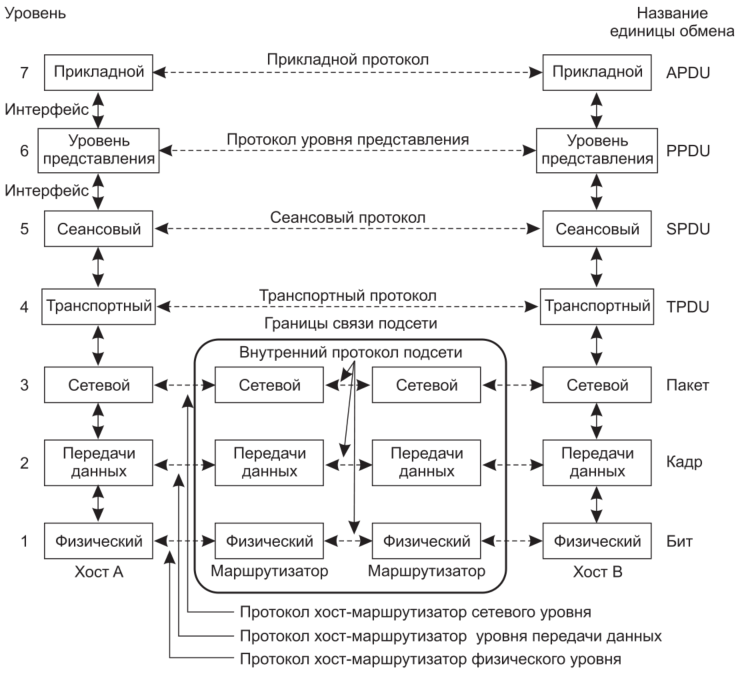
\includegraphics[width=0.9\textwidth]{osiStack.png}
    \attribution{Э. Таненбаум}
\end{center}

Подробнее о том, за что отвечает каждый уровень, немного потом, но обратите внимание, что первые три уровня работают на уровне \textit{подсети}, то есть фрагмента сети, который независимо администрируется и имеет свои локальные сетевые адреса. Только протоколы начиная с транспортного уровня знают, что связанных сетей может быть много, и собственно, только они знают про интернет. Ещё можно обратить внимание, что каждый уровень передаёт данные, которые даже по-разному называются. Физический уровень работает непосредственно с битами, канальный (или <<передачи данных>> на картинке) --- с кадрами (набор бит передаваемой информации плюс, возможно, информация для коррекции ошибок и служебная информация), сетевой --- с пакетами (это кадр плюс метаинформация, нужная для маршрутизации внутри сети). Компьютеры в сети называются \textit{хостами}.

Про модель OSI рассказывают в каждом уважающем себя курсе про сети как про некоторую идеальную архитектуру сетевых протоколов, но на практике она не используется. В современном интернете используется четырёхуровневая модель стека протоколов TCP/IP:

\begin{center}
    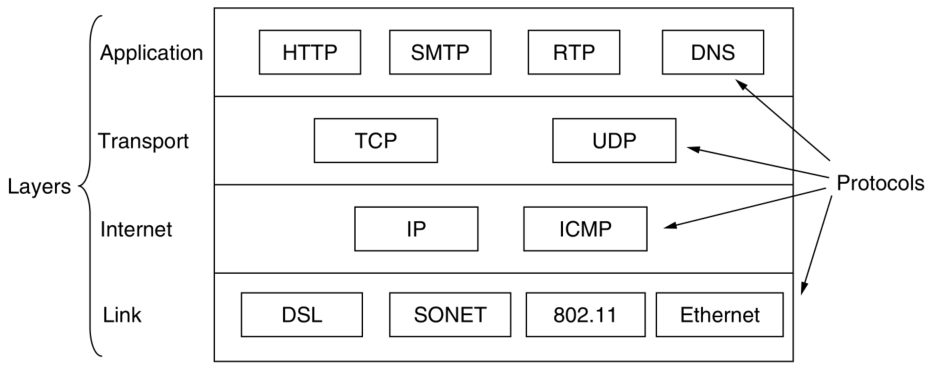
\includegraphics[width=0.9\textwidth]{tcpIpStack.png}
    \attribution{Э. Таненбаум}
\end{center}

Она проще и позволяет иметь протоколы, покрывающие потребности сразу нескольких уровней OSI, что делает реализацию сетевого стека несколько более удобной, при этом не сильно портя архитектуру. Тем не менее, дальше мы рассмотрим уровни стека OSI, потому что они более аккуратно разделяют ответственность, и TCP/IP более-менее хорошо ложится на модель OSI, с некоторыми оговорками.

\subsection{Физический уровень}

Физический уровень содержит протоколы, определяющие физическую передачу данных по какой-либо среде. Протоколы задают, как кодировать передаваемые биты в зависимости от выбранной среды передачи. Надо понимать, что по соображениям эффективности передаётся не каждый бит отдельно, а сразу пачка --- например, Ethernet-оборудование позволяет различать десятки разных уровней электрического напряжения в кабеле, так что можно передавать за один раз несколько битов (единственное, что скорость приходится балансировать с помехозащищённостью). Даже на этом уровне протоколы могут быть весьма хитры и включать в себя коррекцию ошибок физической среды, продвинутые механизмы кодирования/декодирования, разрешения конфликтов передачи, вопросы времени и его синхронизации между устройствами (что тоже сложная задача, иначе отправитель будет думать, что отправил один бит, а получатель --- что принял два, просто одинаковых; речь идёт о микросекундных временных интервалах, так что просто секундомером проблемы не решаются, приходится кодировать сигнал так, чтобы в нём можно было различать такты передачи, подробности в Танненбауме). Зато протоколы физического уровня занимаются только прямой передачей данных от одного устройства к другому, от сетевой карты до сетевой карты. Впрочем, для сред передачи типа мощного радиоканала (например, LTE) это тоже совсем непросто, потому что в эфире в области досягаемости могут находиться сотни устройств и надо сделать так, чтобы они не мешали друг другу.

Примеры протоколов физического уровня:

\begin{itemize}
    \item всем известный Ethernet (<<витая пара>>, который давно уже не пара, но всё ещё витая из соображений помехозащищённости); обычно это восьмижильный кабель со скоростью передачи порядка ста мегабит или гигабита и дальностью передачи порядка 100 метров; имеет интересную историю, посмотрите в Танненбауме;
    \item USB --- да, это тоже протокол физического уровня, позволяющий использовать четырёхжильные пятивольтовые провода для одновременного питания и передачи данных с нескольких устройств одновременно;
    \item xDSL --- например, телефонный ADSL-модем, использующий высокие частоты для передачи данных по обычной телефонной линии. Работает так себе, поскольку телефонные линии обычно не рассчитаны на частоты выше 16КГц (а старые телефонные линии, коих большинство, и в голосовом-то диапазоне работают плохо), так что шумы от низкокачественных проводов изрядно просаживают скорость передачи. Зато не требуется никакая дополнительная проводка, если уже есть телефон, поэтому ADSL исторически был первым и очень популярным способом предоставления (относительно) широкополосного доступа в интернет.
    \item Bluetooth --- основной протокол Personal Area Network, радио с типичной дальностью передачи от 5 до 20 метров, из-за низкого энергопотребления прекрасно подходит для носимой электроники, беспроводной периферии и т.п. Бывают Bluetooth-устройства с дальностью передачи до 100 метров, но на таких дистанциях они конкурируют с WiFi, поэтому редкость.
    \item WiFi (также известный как семейство протоколов IEEE 802.11) --- радио с типичной дальностью передачи порядка 100 метров (с довольно высокими частотами, 2.4 или 5 ГГц, поэтому WiFi хорошо блокируется стенами и прочими препятствиями, так что дальности в помещении и в чистом поле могут различаться на порядки) с пропускной способностью порядка гигабит в секунду (наиболее типичны сейчас адаптеры 802.11ac, но вообще вариантов стандарта очень много). Радиоканалы сильно отличаются от проводных влиянием помех и тем, что разные устройства активно мешают друг другу, особенно это касается WiFi, когда в типичном многоквартирном доме в зоне досягаемости может быть больше десятка точек, активно конкурирующих за каналы передачи. Поэтому WiFi, в отличие от Ethernet, включает продвинутые механизмы коррекции ошибок уже физическом уровне.
    \item SONET (Synchronous optical networking) --- лазерная оптоволоконная сеть, прямая противоположность WiFi в плане физических характеристик канала. Здесь помехи в принципе невозможны, а вероятность ошибки при передаче столь низка, что передаётся только контрольная сумма и при необходимости выполняется повторный запрос, это оказывается быстрее, чем выполнять избыточное кодирование. И дальность передачи без необходимости ретрансляции составляет до 50 километров, при скоростях передачи до 50 терабит в секунду. Что делает оптоволокно идеальным носителем для магистральных каналов. Правда, у него есть проблема --- повреждённый оптоволоконный кабель можно спаять, но это сразу ухудшит характеристики линии на 10\%. Оптоволокно иногда используют и для оконечных линий (<<Ростелеком>> предлагал домашний интернет по оптоволоконной линии по цене 550 рублей в месяц), но пока это дороговато.
    \item Спутниковые протоколы связи --- радио, чисто физически работает медленно, поскольку большинство спутников связи находятся на геосинхронной орбите, высотой 36 тысяч километров над уровнем моря, что даёт заметную (по компьютерным меркам) задержку даже просто по соображениям скорости света. Поэтому нынче пытаются строить сети низкоорбитальных спутников (которые имеют ещё и очень важное преимущество в количестве энергии и размерах антенны для устойчивой связи), но у них очень ограниченная зона покрытия, поэтому их нужно очень много (что огорчает астрономов и создаёт угрозу столкновения с чем-нибудь существенно более дорогим и полезным). И они очень быстро движутся относительно поверхности, так что приходится решать массу интересных вопросов типа передачи открытого соединения от спутника к спутнику и доставки сообщения от спутника по цепочке его собратьев к наземному центру.
    \item Мобильные протоколы в разных вариациях (GSM, EDGE, LTE и т.д.) --- тоже, разумеется, радиопротоколы, со всеми вытекающими последствиями типа беды с помехами и необходимостью делать так, чтобы устройства не мешали друг другу (для чего разные протоколы применяют разные стратегии, типа динамического разделения между устройствами временных слотов для передачи, чем занимаются базовые станции).
    \item Голубиная почта. Канал, где передаваемый пакет печатается на бумажку и привязывается голубю на лапку. Практика показывает, что такой физический канал передачи данных вполне позволяет реализовать протоколы более высокого уровня, правда пинги порядка 6166000 миллисекунд делают его не очень практичным для большинства применений. См. RFC 1149 <<IP over Avian Carriers>> (\url{https://tools.ietf.org/html/rfc1149}).
\end{itemize}

\subsection{Канальный уровень}

Канальный уровень отвечает за общение уже на логическом уровне соединённых напрямую физическим каналом устройств (point-to-point). На этом уровне решаются вопросы коррекции ошибок физического уровня (коды Хэмминга, Рида-Соломона, свёрточные коды и прочая алгебра с теорией чисел), повтора передачи пропавших данных, вопросы использования канала связи (чтобы несколько устройств не мешали друг другу), управления скоростью передачи. Последнее особенно важно, потому что разные сетевые устройства имеют разную скорость работы, и было бы не очень хорошо, если бы отправитель слал пакеты быстрее, чем получатель успевает их хотя бы прочитать. Тут возникает что-то вроде задачи производителя-потребителя, осложнённой тем, что коммуникация между отправителем и получателем не мгновенна и мы не можем дожидаться подтверждения обработки каждого пакета, потому что это было бы слишком долго. Протоколы канального уровня работают уже не в терминах битов, а в терминах фреймов (или кадров) --- блоков по несколько сотен (или тысяч) байтов, снабжённых избыточными кодами.

Пример протокола канального уровня --- PPP (Point to Point Protocol). Этот протокол вводит понятие MAC-адреса --- глобально уникального адреса сетевого устройства (например, D8-FB-5E-E5-55-67), который позволяет послать пакет в среду передачи данных, и устройство с таким MAC-адресом поймёт, что пакет предназначен именно ему. С глобальной уникальностью у MAC-адресов складывается не всегда, но на самом деле требуется только, чтобы в зоне прямой передачи между устройствами все MAC-адреса были различны. MAC-адреса используют маршрутизаторы, чтобы понять, по какому конкретно исходящему порту посылать пакет --- при регистрации на маршрутизаторе устройство сообщает ему свой MAC, в ответ маршрутизатор назначает ему IP-адрес и сохраняет у себя данные, на каком порту и с каким MAC-адресом находится устройство с таким-то IP-шником. Ещё на канальном уровне появляется понятие LLC (Logical Link Control) --- заголовок, в котором хранится тип протокола более высокого уровня, чтобы получатель знал, какой обработчик для входящего сетевого пакета ему вызвать.

\subsection{Сетевой уровень}

Сетевой уровень занимается передачей пакетов по сети из нескольких устройств, где вовсе не обязательно, что каждое устройство непосредственно соединено с другим. Задачи, решаемые сетевым уровнем --- это прежде всего маршрутизация пакета внутри сети (роутинг), передача пакета по сетям разной физической природы. Роутинг интересен тем, что требуется в реальном времени найти оптимальный по тем или иным критериям маршрут для пакета из точки А в точку Б по графу из сетевых устройств, каждое из которых независимо решает задачу роутинга, при этом ещё и не обладая полной информацией о топологии сети (просто потому, что интернет большой и непрерывно меняется, адреса всех машин и пути до всех маршрутизаторов хранить на каждом роутере и постоянно обновлять просто невозможно). Фактически, роутинг --- это что-то вроде распределённого алгоритма Дейкстры. Передача по сетям разной физической природы тоже нетривиальна: разные сети имеют разный размер пакета, так что иногда пакет приходится разбирать на пакеты помельче, а потом собирать обратно, при этом пакеты даже в рамках одной передачи вполне могут идти разными путями, так что дойдут до места назначения в разном порядке, некоторые из них потеряются вовсе, а некоторые придут в нескольких копиях.

Пример протокола сетевого уровня --- IP (Internet Protocol), про который мы подробно поговорим дальше. IP вводит понятие IP-адреса --- это что-то вроде логического адреса машины (в отличие от MAC-адреса, физического адреса, который вшит в сетевую карту), уникального в рамках подсети. Бывают глобально уникальные IP-адреса, и чтобы с компьютером можно было инициировать соединение в интернет, у него должен быть глобально уникальный адрес --- так что все сервера в интернете должны иметь уникальный IP. При этом инициатор соединения (например, компьютер клиента) может уникального адреса не иметь, если его адрес уникален в рамках его подсети --- ответ от сервера всё равно ему придёт правильно, об этом заботится маршрутизатор с помощью механизма NAT (Network Address Translation). IP-адрес же используют браузеры, запрашивая веб-страницы, хотя пользователю об этом обычно не говорят --- используются человекочитаемые доменные имена, которые преобразуются в IP-адреса в процессе выполнения запроса с помощью службы DNS (Domain Name Service). На самом деле, DNS --- это фактически распределённая хеш-таблица (глобального масштаба), отображающая доменное имя в IP-шник. IP адреса бывают двух видов --- IPv4, четырёхбайтовые, к которым все привыкли (например, 192.168.0.1), и IPv6, 16-байтовые, которые появились потому, что глобально уникальных IP-адресов на всех стало не хватать (то есть в интернетах больше $2^{32}$ устройств, к которым хочется иметь глобальный доступ).

\subsection{Транспортный уровень}

Транспортный уровень решает проблемы соединения двух устройств по сети. То есть, допустим, пакеты из точки А в точку Б мы доставлять умеем (это делает сетевой уровень), теперь надо понять, как обеспечить надёжность доставки (и обеспечивать ли её вообще), как обеспечить правильный порядок сообщений, передачу сообщений, которые просто по размеру не лезут в один пакет (мы при обсуждении сетевого уровня говорили, что такая проблема возникает при передаче по гетерогенным сетям --- так вот, сетевой уровень чаще всего просто откажется передавать слишком большой пакет, серьёзная логика по разделению на пакеты реализована на транспортном уровне). На этом же уровне реализуется подтверждение получения пакета и повторная отправка при необходимости.

Основные протоколы этого уровня --- TCP (Transmission Control Protocol) и UDP (User Datagram Protocol). TCP --- протокол, предоставляющий абстракцию непрерывного потока данных между отправителем и получателем. То есть с точки зрения программиста можно взять массив байтов и отправить его по сети, TCP сделает всё возможное, чтобы получатель рано или поздно его получил, причём именно таким, каким он был отправлен. TCP решает проблемы разделения передаваемых данных на пакеты, доставки пакетов с повторной отправкой при необходимости, доставки в правильном порядке, борьбы с дубликатами. TCP устанавливает и поддерживает соединение, может детектировать (рано или поздно) его разрыв. Поэтому TCP используется в ситуациях, когда каждый байт сообщения важен --- при передаче файлов, текстовых данных (включая веб-страницы), сериализованных данных (включая данные средств удалённого вызова, в частности, веб-сервисов).

UDP предоставляет программисту абстракцию <<датаграммы>> --- <<конверта>> с данными (обычно очень небольшого размера, максимум до 64Кб, но на практике всего в сотни байт). Датаграмму можно послать на заданный IP-адрес, но никакой гарантии, что она будет доставлена, не делается, соединение не устанавливается (поэтому датаграммы такие маленькие, чтобы они помещались в IP-пакет), не делается гарантий доставки в правильном порядке или доставки без дубликатов. Казалось бы, не очень полезный протокол, однако передача данных по нему может быть в разы быстрее, чем по TCP (за счёт меньшего оверхеда на служебные поля, и главное, отсутствие необходимости подтверждать доставку, управлять скоростью передачи и т.п.). Поэтому UDP активно используется в ситуациях, когда доставка каждого конкретного байта не обязательна, лишь бы большая их часть примерно вовремя дошла. Например, это стриминг видео или музыки --- они всё равно жмутся с потерями, так что отсутствие нескольких датаграмм только немного ухудшит качество воспроизведения, нормальный пользователь ничего не заметит. Многие компьютерные игры тоже используют UDP, используя на стороне клиентов экстраполяцию в случае потери данных (она там всё равно нужна для обеспечения плавности происходящего в игровом мире). В общей сложности на UDP приходится порядка 10\% всего трафика в интернете.

На уровне TCP и UDP появляется понятие <<порт>> --- способ идентифицировать процесс на хосте, которому предназначено сообщение. Протокол IP заботился только о доставке пакета до хоста (примерно как письма до дома), эти протоколы доставляют пакет уже конкретному адресату (раскладывают письма в ящики с номерами квартир).

\subsection{Сеансовый уровень}

Протоколы сеансового уровня в модели OSI занимаются установлением, поддержанием и корректным закрытием соединения между хостами. В стеке протоколов TCP/IP этим занимается уже знакомый нам протокол TCP, так что он занимает два уровня модели OSI одновременно. А вот UDP чисто транспортный протокол. Кстати, работа с соединением опять непростая задача --- например, корректное закрытие соединения (то есть когда оба участника подтверждают, что они завершили передачу и готовы соединение закрыть) в условиях возможной потери пакетов оказывается вообще неразрешимой задачей, поэтому на практике широко используются таймауты. Кстати, надеяться на то, что TCP скажет вам, что соединение разорвано, не стоит --- TCP сам определяет подходящий таймаут для разрыва соединения исходя из параметров канала, и он вполне может оказаться парой часов. И пока таймаут не наступил, TCP честно пытается доставить сообщение. Поэтому можно физически вынуть провод из сетевой карты, немного подождать и вставить его обратно --- вполне возможно, что соединение не будет разорвано и передача продолжится как ни в чём не бывало. В таком поведении нет ничего удивительного, сеть принципиально ненадёжна, так что сетевые протоколы, гарантирующие доставку, должны быть готовы к таким проблемам, как физическая потеря соединения. При программировании сетевых приложений стоит про это помнить и делать поверх TCP свой механизм контроля состояния канала --- например, \textit{heartbeat}, когда машины, даже если не хотят пока ничего передавать, раз в N секунд обмениваются короткими пакетами просто для того, чтобы дать понять, что они ещё живы.

\subsection{Уровень представления}

Протоколы уровня представления отвечают за кодировку и представление передаваемых данных --- шифрование, сжатие, сериализацию/десериализацию. В модели TCP/IP всем этим занимаются протоколы прикладного уровня, например, HTTPS, поэтому обычно этот уровень тоже отдельно не рассматривается. Конкретно протоколы HTTP и HTTPS на самом деле используются как средство для реализации более высокоуровневых протоколов (например, его используют веб-сервисы, общающиеся по протоколу SOAP), так что эти протоколы можно рассматривать не как прикладные, а как уровня представления.

\subsection{Прикладной уровень}

Протоколы прикладного уровня реализуются для каждого конкретного приложения под его конкретные потребности на базе более низкоуровневых протоколов. Многие из них используются вообще одним приложением (например, протокол Telegram), некоторые стандартизованы и поддерживаются очень много кем (например, XMPP, открытый протокол для instant messager-ов). HTTP и HTTPS можно рассматривать как прикладные протоколы, потому что их используют браузеры для получения веб-страниц. Ещё известные протоколы: FTP (File Transfer Protocol) --- протокол передачи файлов, использующийся в файловых серверах; SMTP (Simple Mail Transfer Protocol) --- протокол, позволяющий получать/отправлять электронную почту. Часто используются протоколы прикладного уровня, которые сами используют HTTP или HTTPS для передачи данных --- например, REST (вообще это не протокол, а архитектура сетевых приложений, но она предписывает более-менее конкретный формат запросов-ответов, так что это что-то вроде протокола или, точнее, архитектуры протоколов), SOAP (вот это конкретный протокол общения веб-сервисов).

\section{Технические детали}

\subsection{IP}

Теперь немного технических подробностей о том, как устроены протоколы IP и TCP/UDP, потому что с ними неизбежно придётся столкнуться в реальной жизни. Начнём с подробностей про IP-адреса.

IP-адреса, как уже говорилось, бывают IPv4 и IPv6. IPv4 имеет размер 4 байта, при этом иерархически организован --- младший байт (или младшие байты) означают номер конкретного компьютера в подсети, старшие байты --- номер подсети. Например, адрес 192.168.0.1 --- это машина номер 1 в подсети номер 192.168. При этом нередко обычный роутер имеет свою систему раздачи IP-адресов (сервер DHCP) и определяет свою подсеть, так что понятно, что дать глобально уникальные номера всем подсетям невозможно. Поэтому IP-адреса даже не пытаются быть глобально уникальными --- главное, чтобы внутри подсети каждый компьютер имел уникальный IP-адрес, чтобы роутер знал, кому именно отправлять сообщение. Есть диапазоны адресов, специально зарезервированные для локальных подсетей, к машинам из которых не требуется иметь доступ извне: 192.168.x.x, 172.16-31.x.x (используются для небольших сетей, типа сети квартиры или небольшого офиса), 10.x.x.x (используется для больших подсетей, например, локалки матмеха). Все IP-адреса из этих диапазонов не глобально уникальны, так что если кто-то предлагает вам по такому адресу подключиться, и он не в вашей подсети, он неправ. Ещё есть специальный адрес 127.0.0.1 (на самом деле, все адреса вида 127.x.x.x) ---  loopback (локальный адрес самого компьютера), доступный даже когда у вас нет никаких сетевых устройств. По этому адресу вы можете получать доступ к сетевым приложениям, запущенным локально (причём, фаервол такие подключения обычно игнорирует), так что loopback-интерфейс часто используется для отладки сетевых приложений. 

Есть ещё понятие \textit{маски подсети} --- это битовая маска, определяющая, какие биты адреса считаются номером подсети, какие --- номером компьютера. Например, для подсети 192.168.x.x маска будет 255.255.0.0 (старшие два байта все единицы --- это номер подсети, младшие нули --- это номер машины). Маски используются в сетевых настройках, чтобы разграничивать доступ внутри сети --- машины из разных подсетей не могут общаться напрямую, даже если физически соединены.

IPv6-адрес имеет размер в 16 байт и записывается в виде групп из четырёх шестнадцатеричных цифр, разделённых двоеточием, например 2001:0db8:85a3:0000:0000:8a2e:0370:7334\footnote{\url{https://en.wikipedia.org/wiki/IPv6_address}}. Ведущие нули можно не писать, самую длинную группу из всех нулей можно заменять на ::, например, 2001:db8::1:0:0:1 --- тоже каноничный IPv6-адрес. Сокращать так можно только одну группу (во избежание неоднозначностей, мы ж не записываем явно размер группы). Структура адресов тоже иерархична, старшие байты обозначают номер сети, младшие номер машины, причём вместо масок используются диапазоны адресов: 2001:db8:1234::/48 означает, что первые 48 бит отводятся на номер сети. То есть пример означает диапазон от 2001:db8:1234:0000:0000:0000:0000:0000 до 2001:db8:1234:ffff:ffff:ffff:ffff:ffff.

А вот как выглядит IPv4-пакет, как он передаётся канальным протоколом (то есть PPP в современном интернете):

\begin{center}
    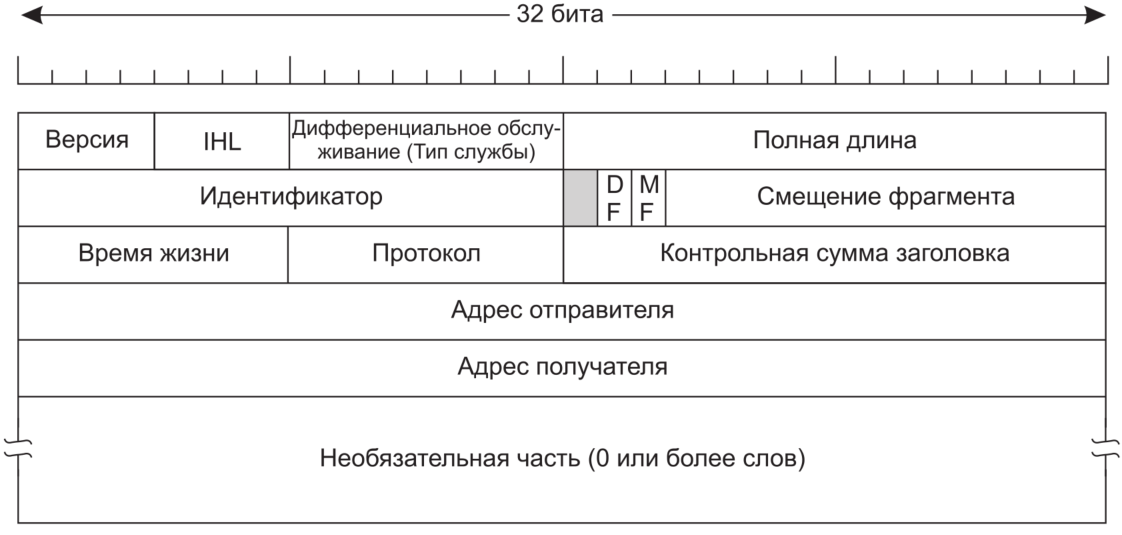
\includegraphics[width=0.9\textwidth]{ipv4.png}
    \attribution{Э. Таненбаум}
\end{center}

\begin{itemize}
    \item Поле <<версия>> содержит номер протокола (4, для IPv6 формат пакета другой).
    \item <<IHL>> (Internet Header Length) --- длина заголовка пакета, её надо передавать, потому что заголовок содержит необязательную часть почти произвольной длины в конце.
    \item <<Дифференцированное обслуживание>> (QoS, Quality of Service) --- насколько приоритетен данный пакет (например, для голосового трафика задержки нежелательны, а потеря пакетов допустима, это обозначается тут).
    \item <<Полная длина>> содержит длину всего пакета.
    \item <<Идентификатор>> --- это просто порядковый номер пакета в сеансе передачи, используется, чтобы бороться с дубликатами и неправильным порядком. Вполне может переполняться и начинаться с нуля в рамах одной передачи, но к тому времени старые пакеты с такими номерами уже успевают протухнуть (Обычно. Для магистральных оптоволоконных линий это потенциально может быть проблемой).
    \item Дальше идёт неиспользуемый бит, такие дела.
    \item Дальше следуют два бита фрагментации --- Dont Fragment и More Fragments (управляют разрезанием пакета на пакеты поменьше).
    \item <<Смещение фрагмента>> --- определяет смещение фрагмента относительно начала целого пакета.
    \item <<Время жизни>> (TTL) --- число проходов через маршрутизаторы, обычно устанавливается в 64 и уменьшается на 1 при каждом роутинге пакета. Когда оно становится равным 0, пакет выкидывается и отправителю посылается обратный пакет о невозможности доставки. Сделано, чтобы пакеты не ходили долго по кругу.
    \item Протокол --- что делать с пакетом, когда он доставлен (это TCP-пакет, UDP-пакет, ещё что-то).
    \item Контрольная сумма заголовка --- думаю, понятно (единственное, что она пересчитывается при каждом роутинге из-за меняющегося TTL).
    \item Адрес отправителя и Адрес получателя --- IP-адреса отправителя и получателя соответственно.
\end{itemize}

\subsection{Порты и сокеты}

Протоколы TCP и UDP вводят понятие \textit{порта}. Порт --- это число от 0 до 65535, идентифицирующее процесс на хосте, которому предназначается сетевой пакет. Например, если компьютеру поступает по сети пакет на порт 80, операционная система вызовет процесс веб-сервера, который должен будет обработать HTTP-запрос и ответить отправителю. Порты привязаны к сетевым интерфейсам и конкретным протоколам, то есть если у вас на компьютере есть две сетевые карты, каждая из них имеет свой IP-адрес и связанный с ним набор портов, причём TCP-порты и UDP-порты --- это разные порты, даже если их номера совпадают (хотя обычно, если приложение использует и TCP, и UDP, оно занимает порты с одинаковыми номерами).

Порты не закрепляются раз и навсегда за каким-то процессом (иначе в мире существовало бы максимум 65536 сетевых приложений), а управляются операционной системой --- процесс может вызвать API сетевого стека ОС и начать \textit{слушать} порт, тем самым прося ОС направлять все пакеты, приходящие на этот порт, ему. Если порт уже занят другим процессом, ОС сообщит об ошибке. Так что в этом смысле порты похожи на файлы. Первые 1024 номера портов зарезервированы под часто используемые нужды, вот некоторые примеры:

\begin{itemize}
    \item 22 --- SSH (Secure SHell), протокол удалённой консоли в UNIX-подобных системах;
    \item 25 --- SMTP, почтовый сервер;
    \item 80 --- HTTP, веб-сервер;
    \item 443 --- HTTPS, веб-сервер по HTTPS (HTTPS --- это HTTP с шифрованием);
    \item 666 --- Doom, один из первых и по сей день весьма популярный 3d-шутер;
\end{itemize}

Если вы хотите написать своё сетевое приложение, выберите просто случайный порт от 1024 до 65535, и если вы планируете написать популярное приложение, желательно погуглить, не использует ли уже кто-то известный этот порт. Потом просто пишете клиенты так, чтобы они делали запросы на этот порт и всё.

При этом неиспользуемые порты чаще всего закрываются на уровне операционной системы (фаервола), подключения на закрытые порты сразу отклоняются и никаких приложений не запускается. Так делается из соображений безопасности, чтобы по сети нельзя было вызвать приложение с известной уязвимостью и получить доступ к хосту (обратите внимание, не нужно, чтобы вас кто-то активно взламывал --- комп может быть атакован давно забытым червём, живущим своей жизнью в локалке). А поскольку обычному ноутбуку или настольному компу незачем принимать входящие соединения, обычно закрыто всё (или почти всё), так что ваше первое сетевое приложение не заработает без манипуляций с настройками фаервола. Впрочем, есть сетевой интерфейс loopback (127.0.0.1), на него фаервол обычно не смотрит (Роскомнадзор один раз добавил 127.0.0.1 в список запрещённых адресов, но быстро исправился). Это всё, как правило, не касается исходящих запросов и ответов на них --- если наш хост инициирует соединение по какому-то известному порту (например, 80), фаервол не возражает. Исходящие порты хоть и используют номера из того же диапазона, обрабатываются обычно отдельно. Исходящие порты часто выбираются случайно при открытии соединения (получатель знает, на какой порт слать ответ, потому что порт отправителя пишется в TCP- или UDP-пакет). 

Порты записываются после IP-адреса через двоеточие, например, 192.168.0.1:80. Браузеры, кстати, понимают такую нотацию, так что если вы хотите сделать HTTP-запрос к конкретному порту, пишите :<номер порта> после URL. Главное, чтобы на этом порту был кто-то, кто может ответить браузеру (то есть поддерживает HTTP).

Ещё есть понятие \textit{сокета} --- это просто программный интерфейс к порту. Сокет можно слушать, сокет можно открыть, в сокет можно писать поток данных (если это TCP-сокет) или слать датаграммы (если это UDP-сокет). Сетевой стек операционной системы позаботится о правильном формировании пакетов и отправке их по сети. Кстати, сетевые стеки --- это довольно большая и сложная часть современных ОС, имеющие иногда неожиданный интеллект. Например, вы думаете, что послали запрос по TCP, но он не ушёл, потому что ОС решила не слать пакет ради тех 10 байт, что вы туда положили, а подождать, пока данных для данного адресата будет побольше (примерно как логистическая компания не повезёт одно яблоко на грузовике, а подождёт, пока грузовик заполнится). К счастью, многими параметрами работы стека можно управлять посредством функций работы с сокетами, но не всеми (таймаутом на разрыв TCP-соединения вроде нельзя, например).

\subsection{NAT}

Итак, для установления сетевого соединения надо знать IP-адрес и порт получателя, и надо, чтобы получатель мог нам ответить. Второе кажется очень простым, мы ведь можем передавать свой <<обратный адрес>> с портом в пакете с запросом. Но вспомним, что IP-адреса не все глобально уникальны, так что если сервер вконтакта, например, получит запрос с адреса 192.168.0.1:35243, то куда ему слать ответ, в мире миллионы машин с таким IPшником.

Всё работает благодаря механизму Network Address Translation (NAT), поддерживаемому роутерами. Работает оно вот так:

\begin{center}
    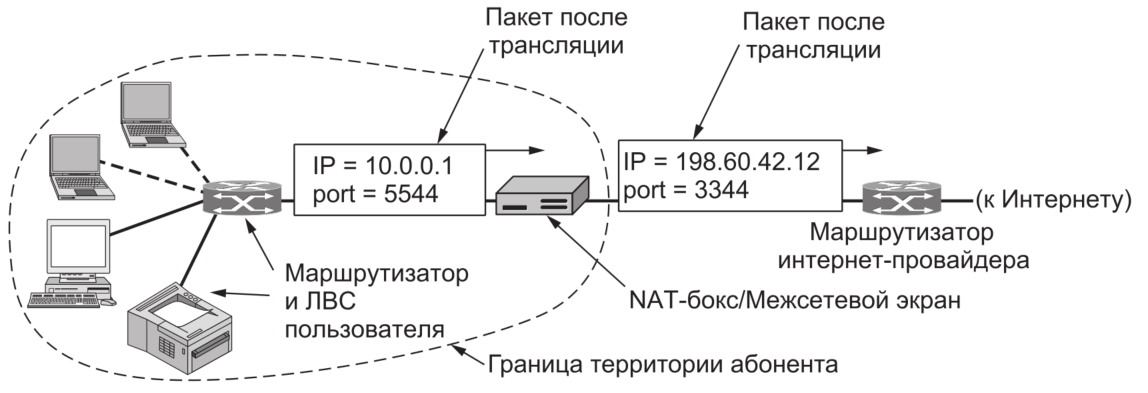
\includegraphics[width=0.9\textwidth]{nat.png}
    \attribution{Э. Таненбаум}
\end{center}

Компьютер в локальной сети без <<настоящего>> IPшника делает запрос, передавая как обычно свой IP-адрес и порт, на котором он ждёт ответ. Роутер со включённым NAT запоминает у себя в таблице эти IP и порт, и вместо IPшника отправителя пишет в исходящий пакет свой IPшник, а вместо порта --- номер ячейки таблицы, в которой он запомнил исходные данные отправителя. Такое преобразование может выполняться несколько раз (например, NAT квартирной сети, находящийся за NATом провайдера), у самого последнего роутера в этой цепочке уже есть выделенный IP. Сервер отвечает по присланному ему обратному адресу, отправляет ответ роутеру, роутер находит сохранённую информацию об отправителе, соответствующим образом модифицирует пакет и отправляет дальше.

Поэтому вообще все машины за NATом получать входящие соединения не могут --- роутер просто не знает, кому они предназначены. Правда, роутеру можно это сказать: что-то в духе <<если на твой IP-адрес придёт запрос на порт 80, отправь его на машину 192.168.0.1 в своей локалке>>. Этот механизм называется \textit{Ports forwarding} и используется, например, если вы купили у провайдера выделенный IP, но хотите иметь в домашней сети несколько компов. Выделенный IP назначается роутеру, нужные порты прокидываются на ваш сервер, стоящий внутри локалки.

Похожая штука --- прокси-сервер. Прокси --- это просто программа, которая пересылает запросы адресату и обычно ещё что-то с ними делает, например, считает потраченный трафик, кеширует запросы и т.п. Прокси могут быть полезными в сетях со странной топологией, где роль роутера играет обычный компьютер с двумя сетевыми картами, либо когда вы хотите контролировать трафик более агрессивно, чем позволил бы обычный роутер.

\subsection{DNS}

Остался нерассмотренным последний и самый важный вопрос сетевого соединения --- откуда узнать IPшник получателя. Это делает сервис DNS (Domain Name Service). DNS представляет собой что-то вроде распределённой адресной книги, которая отображает доменные имена в IP-адреса. Браузер, перед тем, как выполнить запрос к серверу, делает запрос к DNS, передавая ему введённую пользователем адресную строку. DNS-запрос по доменному имени (например, google.com) возвращает IP-адрес (например, 64.233.164.113), только после этого возможен <<настоящий>> запрос. Кстати, обратите внимание, есть URL (например, \url{https://bb.spbu.ru/webapps/portal/execute/tabs/tabAction?tab_tab_group_id=_1_1}), он состоит из имени протокола (https), доменного имени (bb.spbu.ru) и идентификатора ресурса (webapps/portal/execute/tabs/tabAction) с параметрами (tab\_tab\_group\_id=\_1\_1). DNS интересует только доменное имя.

DNS-сервера организованы иерархически. Обычно есть локальный DNS-сервер, поддерживаемый провайдером (обычно их два, основной и дополнительный, чтобы если один помер, сеть продолжала жить). Когда хост делает запрос, он сначала спрашивает у локального DNS-сервера (который хосту указывается при конфигурации сети, либо вручную, либо через DHCP). Если локальный DNS знает такой IPшник, он тут же отвечает, если нет, смотрит на суффикс доменного имени и пытается определить IP-адрес DNS-сервера, который отвечает за этот домен. Например, если bb.spbu.ru ему не известно, он смотрит, не знает ли он адреса DNS-сервера spbu.ru, если знает, пересылает запрос ему, если нет, пересылает запрос на DNS-сервер домена ru. Который сам не знает bb.spbu.ru, но точно знает адрес DNS spbu.ru, поэтому может спросить у него. При этом все ответы запоминаются, так что если мы второй раз запросим bb.spbu.ru, нам тут же ответит локальный DNS-сервер. Есть корневые DNS-сервера\footnote{\url{https://www.iana.org/domains/root/servers}}, отвечающие за домен <<.>> (они обязаны знать про национальные домены, .com, .org и т.д.), но прописывать их как предпочитаемые DNS-сервера у себя в браузер --- плохая идея. Есть ещё общеизвестные DNS-сервера, которые можно использовать, если у вашего провайдера DNS отказал (например, Google Public DNS, с запоминающимся IPшником 8.8.8.8). По моему опыту до половины времени, когда <<нет интернета>>, связано с отказом DNS и легко фиксится указанием известного стороннего сервера. Единственное, для каждодневного использования он не подходит --- если \textbf{перед} выполнением любого запроса браузеру надо сделать несколько запросов буквально на другой конец планеты, говорить о быстро открывающихся страницах не приходится.

Есть, кстати, локальная таблица маршрутизации, поддерживаемая операционной системой (мини-DNS с захардкоженными значениями). Например, localhost ресолвится в 127.0.0.1 без всяких DNS-запросов. Теоретически, с её помощью можно переопределить доменные имена, но на моей памяти не разу не приходилось так делать.

\subsection{Полезные консольные команды}

Вот список команд, которые есть в любой нормальной ОС и позволяют диагностировать сеть или что-то с ней поделать. Их должен знать наизусть и уметь пользоваться хотя бы базовыми сценариями любой нормальный программист:

\begin{itemize}
    \item ping --- проверка соединения с указанным IP или доменным именем, показывает время отклика узла. Работает по протоколу ICMP, сетевого уровня, поэтому ничего не знает про порты и попытка попинговать какой-нибудь порт --- хороший способ быть уволенным из приличной софтверной компании. ping --- это самый простой способ проверить, есть ли вообще возможность подключиться к нужной вам машине, проверить packet loss (особенно полезно с ключом -t, <<пинговать, пока не остановят через Ctrl-C>>). Но учтите, что удалённый компьютер имеет право не отвечать.
    \item tracert (traceroute) --- показывает все узлы, через которые шёл запрос со временами их отклика (если они хотят откликнуться). Эта утилита использует поле TTL IP-пакета, последовательно посылая пакеты с TTL 1, 2, 3 и т.д. и собирая ответные пакеты с уведомлением о невозможности доставки. Тем самым строится примерный путь через маршрутизаторы, с IPшниками маршрутизаторов и временем отклика от них. tracert --- это то, что надо запускать, если интернета нет и дело не в DNS, чтобы узнать, кто именно не отвечает --- где-то у вас или у провайдера. При обращении в техподдержку провайдера там будут более счастливы получить лог tracert, где написано, что у них магистральный роутер пакеты по кругу гоняет, чем <<У меня почта не открывается>>. Роутер провайдера, который <<пакеты по кругу гоняет>>, мне пару раз на практике встречался.
    \item ipconfig под Windows, ifconfig под Linux --- узнать всё про локальный сетевой интерфейс (IP-адреса, MAC-адреса, используемые DNS и т.д.). Например, под Windows ipconfig /all расскажет всё, что вы хотели и не хотели знать про сетевые интерфейсы вашей машины (например, может оказаться, что у вас прямо внутри хоста целая мини-локалка, обслуживающая виртуальные машины).
    \item netcat, nc --- позволяет опросить указанный порт или наоборот, прикинуться сервером, работающим по данному порту. Ей можно сказать, что на любое подключение надо отвечать как-то фиксированно, либо посылать файл и т.д. Поэтому она очень полезна для отладки сетевых приложений --- ей можно тестировать клиент, когда у вас ещё нет сервера, и наоборот, сервер, когда нету клиента. Или если всё есть, но клиент выдаёт странные ошибки, попробуйте netcat-ом пообщаться с сервером и проверить, что он реально доступен и адекватно отвечает. Под Windows netcat не входит в стандартную поставку, так что его надо ставить отдельно.
    \item telnet --- открывает TCP-соединение с заданным хостом на заданный порт, куда вы можете писать любые данные, вручную симулируя работу того или иного протокола. Например, можно пообщаться с почтовым сервером GMail (но, правда, от него ничего содержательного не добиться, потому что авторизация и шифрование):
        \begin{minted}{text}
telnet smtp.gmail.com 25
220 smtp.gmail.com ESMTP m71-v6sm2246896lje.84 - gsmtp
HELP
214 2.0.0  https://www.google.com/search?btnI&q=RFC+5321 m71-v6sm2246896lje.84 
- gsmtp
        \end{minted}
        При этом из telnet довольно нетривиально выйти: Ctrl + `]', quit. Под Windows тоже не входит в стандартную поставку, надо ставить отдельно.
\end{itemize}

\section{Работа с сетью в .NET}

Теперь наконец перейдём к тому, что надо писать в коде, чтобы сделать сетевое приложение на <<сырых>> сокетах. В реальной практике чаще приходится пользоваться прикладными протоколами, типа HTTPS --- настолько, что, скорее всего, если вы используете классы, показанные далее, вы либо пишете какую-то низкоуровневую утилиту, игру, или делаете что-то неправильно. Про высокоуровневые механизмы работы с сетью --- в следующей лекции.

Всё, что связано с сетью, в .NET находится в пространстве имён System.Net. Собственно, за работу с сокетами отвечают классы TcpListener, TcpClient, UdpClient. TcpListener позволяет открыть входящий порт и слушать его для установления соединения, TcpClient --- открыть исходящий порт и установить соединение. Протокол UDP не имеет понятия <<соединение>>, поэтому UdpClient умеет и отправлять датаграммы, и принимать их.

Открытым соединением позволяет управлять класс Socket. TcpListener возвращает объект типа Socket, когда соединение установлено. Чаще всего на сервере TcpListener слушает входящие соединения, получает соединение, создаёт Socket и отдаёт его в отдельную асинхронную задачу, продолжая слушать следующие соединения. При установлении соединения открытому сокету назначается новый порт, который он может использовать для общения с клиентом, а исходный порт готов принимать новые соединения, пока первое ещё активно.

Класс Dns отвечает за работу с DNS-службой, а IP-адрес с портом представляет структура IPEndPoint (хотя большинство методов прекрасно понимают IP-адрес в просто строковом формате).

\subsection{TCP}

Вот минимальный пример сервера, слушающего сетевые соединения по порту 8888, и просто печатающего всё, что ему присылают:

\begin{minted}{csharp}
static void Main(string[] args)
{
    const int port = 8888;
    var listener = new TcpListener(IPAddress.Any, port);
    listener.Start();
    Console.WriteLine($"Listening on port {port}...");
    using (var socket = listener.AcceptSocket())
    {
        var stream = new NetworkStream(socket);
        var streamReader = new StreamReader(stream);
        var data = streamReader.ReadToEnd();
        Console.WriteLine($"Received: {data}");
    }
    listener.Stop();
}
\end{minted}

IPAddress.Any --- константа, означающая <<все сетевые интерфейсы>>. Обычно для того, чтобы слушать одновременно все сетевые интерфейсы компьютера, надо права администратора, но иначе вам надо было бы указать IP-адрес конкретной сетевой карты. Порт 8888 был взят просто <<из головы>>, как незанятый. \mintinline{csharp}{listener.Start();} начинает слушать порт, \mintinline{csharp}{listener.AcceptSocket()} блокирует поток до установления соединения. Дальше мы получаем открытый сокет, создаём NetworkStream, который позволяет читать/писать в этот сокет, надеваем на него StreamReader и читаем, как из обычного файла. С той лишь разницей, что у файла есть конец, а у сетевого потока конец --- это закрытое соединение, так что \mintinline{csharp}{streamReader.ReadToEnd();} не вернёт управление, пока клиент не отключится. Обратите на это внимание, это хороший способ прострелить себе ногу --- клиент шлёт серверу команду и ждёт ответ, который сервер никогда не пришлёт, думая, что клиент ещё не закончил передачу команды. Дедлок. Чтобы этого избежать, используют протоколы, где команды можно отличить друг от друга без закрытия соединения --- например, каждое сообщение разделять переводом строки, и читать ReadLine-ом. Но если в самом сообщении может быть перевод строки, то не всё так просто. Поэтому прикладные протоколы не так тривиальны.

Вот как мог бы выглядеть код этого же приложения со стороны клиента:

\begin{minted}{csharp}
static void Main(string[] args)
{
    const int port = 8888;
    using (var client = new TcpClient("localhost", port))
    {
        Console.WriteLine($"Sending to port {port}...");
        var stream = client.GetStream();
        var writer = new StreamWriter(stream);
        writer.Write("Hello, world!");
        writer.Flush();
    }
}
\end{minted}

Конструктор TcpClient сам открывает соединение и возвращает управление, когда оно установлено. Тут мы делаем запрос к локалхосту (так что это приложение не очень полезно как сетевой чатик) на порт 8888, тот самый, который сервер слушает. Опять-таки, получаем стрим, StreamWriter-ом записываем в него строку, командой \mintinline{csharp}{writer.Flush();} говорим, что сообщение закончено и его можно отправить, и закрываем соединение.

Один и тот же сокет может использоваться и для чтения и для записи, позволяя реализовать полноценное общение между клиентом и сервером. Серверная часть:

\begin{minted}{csharp}
static void Main(string[] args)
{
    const int port = 8888;
    var listener = new TcpListener(IPAddress.Any, port);
    listener.Start();
    Console.WriteLine($"Listening on port {port}...");
    using (var socket = listener.AcceptSocket())
    {
        var stream = new NetworkStream(socket);
        var reader = new StreamReader(stream);
        var data = reader.ReadLine();
        Console.WriteLine($"Received: {data}");

        Console.WriteLine($"Sending \"Hi!\"");
        var writer = new StreamWriter(stream);
        writer.Write("Hi!");
        writer.Flush();
    }
    listener.Stop();
}
\end{minted}

И клиентская: 

\begin{minted}{csharp}
static void Main(string[] args)
{
    const int port = 8888;
    using (var client = new TcpClient("localhost", port))
    {
        Console.WriteLine($"Sending \"Hello!\" to port {port}...");
        var stream = client.GetStream();
        var writer = new StreamWriter(stream);
        writer.WriteLine("Hello!");
        writer.Flush();

        var reader = new StreamReader(stream);
        var data = reader.ReadToEnd();
        Console.WriteLine($"Received: {data}");
    }
}
\end{minted}

Обратите внимание, что всё должно происходить в правильном порядке --- мы сначала ждём сообщение от клиента, затем посылаем ему ответ. Если и сервер, и клиент будут ждать сообщения, всё опять задедлочится. Кроме того, пока обслуживается один клиент, остальные ждут. С этим может помочь побороться механизм async/await из прошлой лекции, вот первый шаг к многопоточному серверу:

\begin{minted}{csharp}
static async Task Main(string[] args)
{
    const int port = 8888;
    var listener = new TcpListener(IPAddress.Any, port);
    listener.Start();
    Console.WriteLine($"Listening on port {port}...");
    using (var socket = await listener.AcceptSocketAsync())
    {
        var stream = new NetworkStream(socket);
        var reader = new StreamReader(stream);
        var data = await reader.ReadLineAsync();
        Console.WriteLine($"Received: {data}");

        Console.WriteLine($"Sending \"Hi!\"");
        var writer = new StreamWriter(stream);
        writer.AutoFlush = true;
        await writer.WriteAsync("Hi!");
    }
    listener.Stop();
}
\end{minted}

На самом деле, ничего не поменялось, потому что Main своего цикла обработки событий не имеет и запускается только один раз, так что тут сервер тоже заблокируется на AcceptSocketAsync. Поэтому сделаем более правильно:

\begin{minted}{csharp}
static async Task Main(string[] args) {
    const int port = 8888;
    var listener = new TcpListener(IPAddress.Any, port);
    listener.Start();
    Console.WriteLine($"Listening on port {port}...");
    while (true) {
        var socket = await listener.AcceptSocketAsync();
        Task.Run(async () => {
            var stream = new NetworkStream(socket);
            var reader = new StreamReader(stream);
            var data = await reader.ReadLineAsync();
            Console.WriteLine($"Received: {data}");

            Console.WriteLine($"Sending \"Hi!\"");
            var writer = new StreamWriter(stream);
            await writer.WriteAsync("Hi!");
            await writer.FlushAsync();

            socket.Close();
        });
    }
}
\end{minted}

Тут AcceptSocketAsync тоже только для красоты, но всё, что может быть асинхронным, должно быть асинхронным. Потому что, например, сервер может быть переиспользован в графическом приложении, и вот там AcceptSocketAsync уже сильно поможет. А вот Task.Run с асинхронной лямбдой (кстати, лямбды бывают асинхронными, как и обычные методы) тут очень по делу. Каждый клиент обслуживается в своём потоке на тредпуле, причём, поскольку лямбда асинхронная, длительные операции чтения не блокируют этот поток и не мешают работать другим задачам в пуле. При этом основной поток готов принимать следующего клиента, которого можно поставить в другой поток на пуле, так что такой сервер может обслуживать одновременно довольно много желающих (не больше 65536, правда --- из-за ограниченности количества портов).

А вот так примерно можно сделать полностью асинхронный сетевой чат, где клиент и сервер могут в произвольном порядке обмениваться сообщениями:

\begin{minted}{csharp}
private static async Task Main(string[] args) {
    ...
    while (true) {
        var client = await listener.AcceptTcpClientAsync();
        Writer(client.GetStream());
        Reader(client.GetStream());
    }
}

private static void Writer(NetworkStream stream) {
    Task.Run(async () => {
        ...
    });
}

private static void Reader(NetworkStream stream) {
    Task.Run(async () => {
        ...
    });
}
\end{minted}

Внутри Writer и Reader могут работать асинхронные бесконечные циклы, вычитывающие данные из сети и печатающие их на консоль, либо наоборот, читающие данные с клавиатуры и пишущие в сокет. Например, как-то так:

\begin{minted}{csharp}
private static void Writer(NetworkStream stream)
{
    Task.Run(async () =>
    {
        var writer = new StreamWriter(stream) { AutoFlush = true };
        while (true)
        {
            Console.WriteLine(">");
            var data = Console.ReadLine();
            await writer.WriteAsync(data + "\n");
        }
    });
}
\end{minted}

\subsection{UDP}

Работать с протоколом UDP внешне гораздо проще. Вот минимальный UDP-сервер:

\begin{minted}{csharp}
static async Task Main(string[] args)
{
    const int port = 8888;
    var udpClient = new UdpClient(port);
    Console.WriteLine($"Listening on port {port}...");
    var received = await udpClient.ReceiveAsync();
    var data = Encoding.UTF8.GetString(received.Buffer);
    Console.WriteLine($"Received: {data}");
}
\end{minted}

udpClient.ReceiveAsync просто вернёт нам датаграмму, как только она придёт, никаких сокетов, никаких соединений. А вот со стороны клиента: 

\begin{minted}{csharp}
static async Task Main(string[] args)
{
    const int port = 8888;
    var udpClient = new UdpClient();

    Console.WriteLine($"Sending \"Hello!\" to port {port}...");
    var data = Encoding.UTF8.GetBytes("Hello!");
    await udpClient.SendAsync(data, data.Length, "localhost", port);
}
\end{minted}

Тут мы пользуемся тем же UdpClient, и даже не говорим ему порт при создании --- при отправке датаграммы указываем и IP (точнее, тут вообще доменное имя, оно само превратится в IP через DNS), и порт. Существенно проще, чем TCP.

Но, как уже говорилось, UDP не даёт никаких гарантий по доставке сообщений или доставке только одной копии сообщения. И если вы хотите передать сообщение размером больше, чем одна датаграмма, вам надо будет самостоятельно разобрать сообщение и правильно собрать (с учётом, что что-то не дойдёт вообще, что-то придёт дважды-трижды, а что-то придёт секунды через две после всего остального). А размер датаграммы, хоть и теоретически порядка 65535 байт, на практике не должен быть больше 508 байт, иначе многие роутеры такой пакет не пропустят. 

Вообще, на UDP можно построить надёжный протокол коммуникации, вручную введя идентификацию сообщений, подтверждения доставки и повторы, но зачем, если есть TCP. Так что передавать по UDP информацию, где важен каждый байт (например, любые файлы) --- очень плохая идея.

\end{document}
